\documentclass{article}


\usepackage[utf8]{inputenc}
\usepackage[english]{babel}
\usepackage{biblatex}
\usepackage{graphicx}
\usepackage{mathbbol}
\addbibresource{biblio.bib}
\bibliography{biblio}


\title{Visualisation of big graphs}
\author{Flora Helmers, Mahsa Niazi}
\begin{document}
\maketitle

\section*{Introduction}
Linked data is a concept that is extending itself nowadays. Now data is not only stored in tables, but also in the form of a graph. One example could be a social network, described by its users (the nodes) and their connexions (the edges). Data scientists can extract information from these datasets, by connnecting their machine to specific endpoints and using the domain-specific language SPARQL, which is like SQL but for graphs. This make these datasets unaccessible to the average person. Therefore we would like to offer a visualisation of these datasets, in order to allow people to explore them. 

The graphs are huge. A small one is defined as having less than 100k edges. Therefore a standard library, such as networkx in python, cannot be used.
The graphs are also non planar, which make the visualisation in 2D not very readable. 
Also having a 3D representation allows a better immersion inside the data and the possibility to follow each of the edges outgoing from a node.

So the goal is to create a visually pleasing graph on a 3D map. This means defining a layout, ie the position of each nodes on $\mathbb{R}^3$. After that we can simply use the c++ library polyscope to visualize them. 

The estetically pleasing layout are called force oriented. There exist many algorithms to draw graphs in 2D. But far less exist to draw large graphs in 3D. Therefore we use the GRIP algorithm proposed by Gajer and Kobourov in \cite{gajer00} that was conceived for graphs of size 30k nodes. It is not a lot, but it already allows to see interesting things.


\section{Structure of the code}

\begin{figure}[h!]
    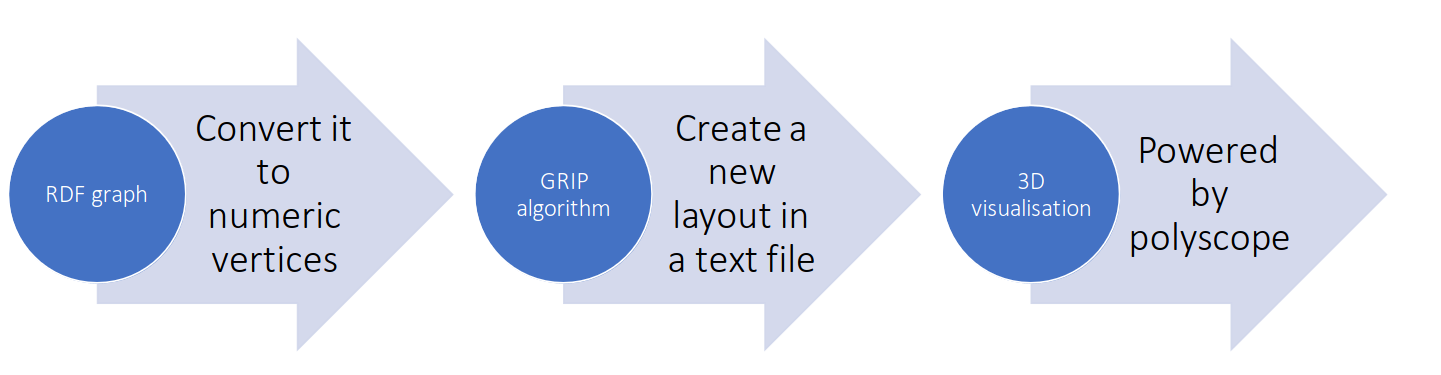
\includegraphics[width=\textwidth]{process.png}
    \caption{Overview of the process}
\end{figure}

The original format of the file is the one of the knowledge graph (it's the name of the graph of data mentionned above). A knowledge graph is described by a triple (subject, object, predicate). There exist many serialisation format to express these triples. But for us, it means that the construction of the graph will be at least linear in the number of triple. Small datasets are made of less than 100k triples. Transforming it in the numeric format is possible, if we put the limit of INT\textunderscore MAX, else we could consider using the type double. We store the graph in the form of adjacency lists. If there are several edges between a pair of vertices, we consider them has being one, because we can play on this parameter afterward in the visualisation. 

The code is splitted in two parts. The first one is the part of the algorithm written in c++. The second is the visualisation part written in python. This heterogeneity can be explained by the authors.

 


\section{Visualisation}
With a random layout, the graph still can be estetically pleasing with great chrome effect. 
\begin{figure}[h!]
    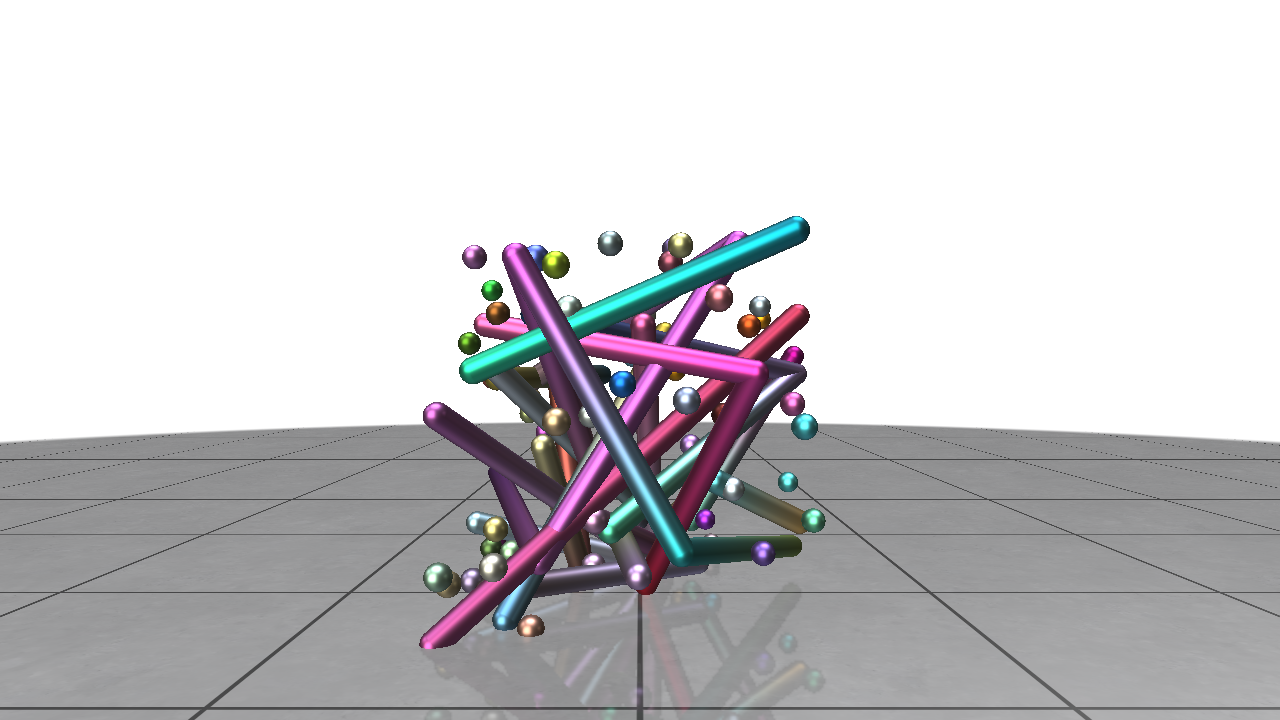
\includegraphics[width=10cm]{random_generator.png}
\end{figure}
The structure used in polyscope is the curve network one.

\section{The grip algorithm}

Presented in \cite{gajer00}.
\begin{figure}[h!]
    \includegraphics[width=10cm]{pseudo_algorithm.png}
    \caption{Summary of the algorithm from \cite{gajer00}}
\end{figure} 

\subsection{The preprocessing : computing the distances in the graph}
The function $dist_{G}$ is called many times in the algorithm. At least one time for every vertices. Therefore, it is necessary to have the matrix of the distances of all pair of vertices. In order to do so, we need to store the values.In order to divide the size of storage by two, we only the store the superior triangle of the matrix. 
In order to compute the distances, we use the Floyd-Warshall algorithm in $O(nbVertices^3)$. We could optimise this computation by assuming that knowledge graph are sparses, and by using Johnson's algorithm.  

For Floyd Warshall algorithm, we use the macro INT\underscore MAX instead of defining a type for infinity. INT\underscore MAX equals 2,147,483,647. It reminds that since vertices are int, their number is limited to 2M. This is a hint that the algorithm can't be scaled to medium knowledge graphs (where the number of triples is between 1M and 100M triples). 


\subsection{The filtration}
There are two filtrations proposed in the article. 
The first is the Center Graph filtration (CG) and the second is the maximal independent set filtration.
Due to time constraints, we implemented the first but not the second. 

Both necessitates call the graph distance. Therefore the Floyd-Warshall algorithm is applied on the graph as a part of preprocessing. 

The construction of the filtration sets is recursive.
First element of $V_{k}$ is chosen randomly. 
Then the farthest element from the set is added at each iteration. 
We define the farthest element from the set as 
$argmax_{u \in G} dist(u, V_{k})$
where the distance to a set is defined as $dist(u, V_{k}) = min_{v \in V_{k}} dist(u, v)$
it can be found in O($ max(|V_{k}|, |V|)$). 

An optimization can be added which is based on the idea that vertices are selected in exactly one set. Instead of iterating on all vertices in the function getFarthestVertex, we iterate only on the ones that have not been selected yet. TODO

\subsection{Find the initial position}
To do so we use graph distance to map it on the Euclidean space \mathbb{R}. The idea is to keep the equidistance to the three closest nodes as described in \cite{gajer00}. 
We adapt it to 3D space. 
In 3D, two spheres can have 4 intersections points (to be proven).
As proposed in \cite{gajer00},  we find them by solving the three equations : 
$dist_{R}(u, t) = dist_{G}(u, t)$
$dist_{R}(v, t) = dist_{G}(v, t)$

The method to solve these quadratic equations is ?? 

TODO

Then we sekect one point from each solution such that the distance between them is minimal (how to define that). 
def 1 : $distmin(A, B, C) = argmin_{a \in A, b \in B, c \in C}  dist(a, b) + dist(b, c) + dist(c, d)$
check problematic cases : what if we don't have a triangle.
because we have as hyp, that the points are all belonging to a sphere with different center. Then we have a clean triangle. 


Note: the positions are computed in float, and then we add the right granularity when creating the OBJ file. The diameter is there a useful parameter. 

Then we take the barycenter of each element. 

To compute the intersection between two spheres $\mathcal{S}_{u} = \mathcal{S}(u, r_{u})$ and $\mathcal{S}_{v} = \mathcal{S}(v, r_{v})$ where $u$ and $v$ are in $\mathbb{R}^3$ :
we want to find the points (x, y, z) in \mathbb{R}^{3} such that it belongs to $\mathcal{S}_{u}$ and $\mathcal{S}_{v}$. 
A point belongs to $\mathcal{S}_{u}$ iff : 
$ (x-u_{x})^2 + (y - u_{y})^2 + (z - u_{z})^2 = r_{u}$
which is equivalent to \\
$x^2+ y^2+z^2 - 2 (x * u_{x} + y * u_{y} + z * u_{z}) = r_{u} - ||u||$
Same for $\mathcal{S}_v$.  
By subtracting the equations for $\mathcal{S}_u$ and $\mathcal{S}_v$, we obtain the equation of a plane. 
equation of a plane : 
$x(u_{x} - v_{x}) + y (u_{y} - v_{y}) + z (u_{z} - v_{z}) = \frac{1}{2} (r_{v} - ||v|| - r_{u} + ||u||)$
When knowing x and y, we can compute z. (Isn't it a problem in terms of conditions?)

In Coope's article on the intersection of n sphère \cite{nsphere}, it can be seen that there are at most two points in the intersection between three sphere in $\mathbb{R}^3$. 

Since we are in a plane, we can go back to the case where we had two 2D circles.  
https://math.stackexchange.com/questions/256100/how-can-i-find-the-points-at-which-two-circles-intersect proposition

an approximation


\paragraph{Finding closest neighbours}
We do a bubble tri. 



\section{Future work}
This project has allow us to think about diverse problems. A geometrical problem : the intersection of the spheres. But also technical problems like what data structure to use when we have in mind the visualisation of huge graphs.


\subsection{Time and emory optimisation}
The memory taken by the adjacency matrix could be divided by 2. Our adaptation of the algorithm doesn't reach the lower bound expected. 

The time could be also rethought by using parallel programmation. 


\subsection{Playing with the distances}
Then playing on the initial matrix. Eg on the initial Floyd-Warshall make a weight on the matrices depending on the value of the predicates they have. These could allow to vary the perspectives.

\printbibliography[
heading=bibintoc,
title={Bibliography}
]
\end{document}